\chapter{SheepOS的启动过程}
\label{cha:OSboot}

\section{相关概念简介}

与系统启动相关的模块主要涉及BIOS、MBR、Loader、Kernel等部分。在操作系统
启动过程中,先由BIOS来找到MBR,然后由MBR来引导并加载Loader,再
由Loader来加载Kernel。本节我们先简要介绍一下上述概念,然后再详细剖析
SheepOS的启动过程。

\subsection{基本输入输出系统(BIOS)}
\label{sec:BIOS}

BIOS的全称是Basic Input/Output System,意思就是基本输入输出系统。它是计
算机上第一个运行的软件。当然,它不可能自己加载自己,那么它就只能是由硬
件来加载了,而这个硬件就是CPU\cite{zg2016}。在计算机通电
瞬间,如图\ref{fig:img2-1}所示,寄存器\texttt{CS:IP}会被赋予一个初
值:\texttt{F000:FFF0}。之后,CPU将会执行下面这条指令:
\begin{codeblock}
\begin{nasmcode}
jmp f000:e05b
\end{nasmcode}
\end{codeblock}
\texttt{JMP},顾名思义就是要跳转到内存中的\texttt{F000:E05B}这个地址,
这里就是BIOS待机的地方。\texttt{JMP}到这之后,BIOS被唤醒,接管了CPU的使用权
。之后BIOS要做的事情就是:
\begin{itemize}
\item 准备好和基本输入输出相关的函数
\item 检查硬件
\item 将主引导扇区(MBR)的代码加载到内存中的\texttt{0x7C00}位置
\item 跳转到\texttt{0x7C00}
\end{itemize}

\begin{figure}[H]
  \centering
  \includegraphics[width=.9\linewidth]{图2-1}  
  \caption{Bochs屏幕截图}
  \label{fig:img2-1}
\end{figure}

\subsection{MBR的工作}
\label{sec:MBR}

MBR,全称是Master Boot Record,主引导扇区,共有512个字节,其结构如图\ref{fig:mbr}所
示。主要由三个部分组成,分别是:
\begin{itemize}
\item 主引导程序(Bootloader):占扇区前446个字节,在计算机开机,BIOS完成自检后,会将MBR加载
  到内存中,然后执行前446字节的引导程序。
\item 硬盘分区表(DPT):占扇区中间64个字节,主要用来定位各个分区,访问用户数据。
\item MBR结束标志\texttt{0xAA55}:占扇区最后2字节,也被称为魔数。每次执行引导程序时都会检查
  程序的结尾是否是\texttt{0xAA55},若不是的话则会认定这是一个无效的MBR引导扇区,将会中止引
  导。
\end{itemize}

\begin{figure}
  \centering
  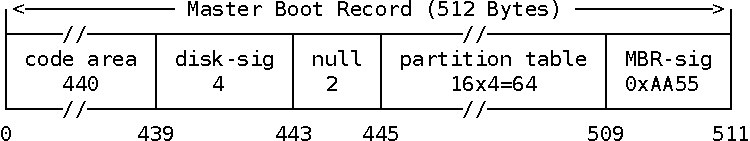
\includegraphics[width=.7\textwidth]{mbr}
  \caption{MBR的结构}
  \label{fig:mbr}
\end{figure}

BIOS在\texttt{0x7C00}处把CPU的控制权交由MBR之后,将会再次进入待机状
态,至此,BIOS的任务就完成了。\texttt{MBR.S}中的代码部分是由自己编写的,它可
以简单到只要如下三条汇编程序语句:%
\begin{itemize}
\item 告诉汇编器把MBR的起始地址编译为\texttt{0x7C00};
\begin{codeblock}
\begin{nasmcode}
 SECTION MBR vstart=0x7c00
\end{nasmcode}
\end{codeblock}
\item \verb'$'表示本行所在的地址,\verb'$-$$'意思是本行到本section的偏移量,MBR必须得填满
  512个字节,而最后两个是固定的\texttt{0x55}和\texttt{0xAA},所以剩下空着的部分用0来填充。
\begin{codeblock}
\begin{nasmcode}
 times 510-($-$$) db 0 
\end{nasmcode}
\end{codeblock}
\item MBR结束;
\begin{codeblock}
\begin{nasmcode}
 db 0x55,0xaa  
\end{nasmcode}
\end{codeblock}  
\end{itemize}

这样就拥有了一个很小的MBR,当然只是这样做的话,屏幕上可能会有很
多乱七八糟的信息,因为Bochs虚拟机的设计师默认是会显示一些Bochs
的版本号等等信息的,所以还是让Bochs的界面能够显示的清爽一些,调
用汇编寄存器\texttt{0x60}号功能号来实现清屏,再通过对字符串的
操作来实现在Bochs界面上打印出来一个\texttt{Hello, OS world!}
来表示MBR已经被成功加载了。代码如下:%

\begin{longlisting}
\begin{nasmcode}
    org 07c00h          ; 告诉编译器程序加载到7c00处
    mov ax, cs          
    mov ds, ax          
    mov es, ax          
    mov ah, 0x6         ; 利用0x60号功能清屏
    mov al, 0x0         ; AL = 上卷的行数(0表示全部)
    mov bx, 0x700
    mov cx, 0x0
    mov dx, 0x184f
    int 10h
    call DispStr        ; 调用显示字符串例程
    jmp $               ; 无限循环
DispStr:
    mov ax, BootMessage
    mov bp, ax          ; ES:BP = 串地址
    mov cx, 16          ; CX = 串长度
    mov ax, 01301h      ; AH = 13,  AL = 01h
    mov bx, 000ch       ; 页号为0(BH = 0) 黑底红字(BL = 0Ch,高亮)
    mov dl, 0
    int 10h             ; 10h 号中断
    ret
BootMessage:        db  "Hello, OS world!"

times   510-($-$$)  db  0   ; 填充剩下的空间,使生成的二进制代码恰好为512字节
dw  0xaa55                  ; 结束标志
\end{nasmcode}
\end{longlisting}

如图\ref{fig:img2-2}所示,一个最小的操作系统就完成了。

\begin{figure}[H]
  \centering
  \includegraphics[width=.7\linewidth]{图2-2}
  \caption{Hello, OS World!}
  \label{fig:img2-2}
\end{figure}

至此,MBR已经从BIOS上接管了CPU的使用权。

\subsection{Loader的工作}
\label{sec:Loader}

MBR在完成跟BIOS的交接后,需要解决三个问题:1)从硬盘上找
到Loader;2)把Loader搬运到内存中的什么地方;3)怎样搬运。其中第1、2条
其实是由自己定义的,可以自己选择把Loader放在硬盘里的任何一个地址,该操作系统中
放在了第二扇区,所以就需要MBR去硬盘的第二扇区寻找Loader。那么找到Loader后
要搬运到哪呢?

\begin{figure}
  \centering
  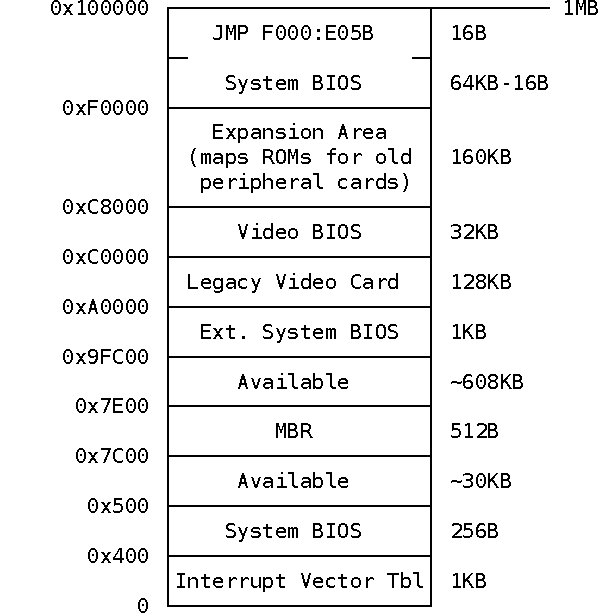
\includegraphics[width=.4\linewidth]{boot-mem}
  \caption{实模式下的内存布局}
  \label{fig:neicun}
\end{figure}

如图\ref{fig:neicun}所示,有两个可用的区
域\texttt{0x7E00~0x9FBFF}和\texttt{0x500~0x7BFF},本操作系统中将它放
在了\texttt{0x900}这个地方,所以最终MBR就会把Loader搬运到\texttt{0x900}这
个地方。

\subsection{内核的启动}
\label{sec:kernel}

\subsubsection{从实模式到保护模式}
\label{subsec:protect}

在Loader被搬运到\texttt{0x900}之后,需要将操作系统由实模式转变到保护模式\cite{LWY2013},原
因有以下几点:
\begin{itemize}
\item 实模式下操作系统和用户程序会属于同一个特权级。
\item 逻辑地址 = 物理地址,顾名思义就是用户程序引用的地址最终都指向真实的物理地址。
\item 用户程序能够自由地修改段基址。
\item 当需要访问超过64KB内存的区域时,要切换段基址。
\item 浪费计算机资源,因为一次只能够运行一个程序。
\item 一共只有20条地址线,加起来最大的可用内存也仅有1MB。
\end{itemize}

所以需要将操作系统引导到保护模式下才可以既安全,又能充分地利用计算机的
资源,还不用过于担心内存问题。

实模式的寻址方式是“(段基址:段内偏移
地址)”的形式;而保护模式的寻址方式是“(选择子:段:偏移地址)”,所以保护
模式还需要段描述符来描述一个段的信息,一个段描述符是8个字节,多个段描述
符就构成了段描述符表也就是“GDT”\footnote{GDT(Global Descriptor Table)\cite{chxs2012},全局描述符表,一个
  CPU对应一个GDT,它可以被放在内存的任何地方,也就是说它是全局的,存放在内存中的某个位置,
  而这个位置将由我们来指定}。因此第一步就是打开A20地址线(详见第\ref{sec:inprotect}节),让操作系
统能够访问更大的空间,方法也很简单,就是把\texttt{0x92}的第一个比特
置1就可以了。代码如下:
\begin{codeblock}
\begin{nasmcode}
in al, 0x92
or al, 0000_0010B
out 0x92, al
\end{nasmcode}  
\end{codeblock}
仅需要3行代码,就可以打开A20地址线。
之后加载之前写好的GDT。
最后一步就是将保护模式的开关 --- \texttt{CR0}寄存器 --- 的\texttt{PE}比特置1,也很简单,就三行代码:

\begin{codeblock}
\begin{nasmcode}
mov eax, cr0
or  eax, 0x00000001
mov cr0, eax
\end{nasmcode}  
\end{codeblock}

至此,操作系统已经成功进入了保护模式,接下来就是把CPU的使用权交给Kernel(内核)。

\subsubsection{内核初始化}

Loader会把内核从硬盘上读出来,然后加载到内存中去,至此,CPU的使用权就会传到内核手上
,这就是操作系统从电脑开机到接管CPU使用权的一个大致过程。内核的代码如下:

\begin{codeblock}
\begin{ccode}
int main(void)
{
    while(1);
}
\end{ccode}  
\end{codeblock}

没错,就可以是这么一个简单的程序,操作系统实质上从头到尾也就是在做这么一件
简单的事情。

\section{SheepOS的启动过程}
\label{sec:booting}

当按下计算机的开机键后,计算机开始自检,之后运行第一个软
件BIOS。BIOS的工作在第\ref{sec:BIOS}节有过介绍,
在BIOS把CPU使用权交给了MBR之后,MBR会在硬盘上的第二个扇区找到
\texttt{Loader.bin}并把它加载到内存中去,之后操作系统将在Loader中跳入
保护模式,并且由Loader来加载内核。

\subsection{读取硬盘扇区}

为了让MBR能够定位Loader,需要一个\texttt{rd\_disk()}函数来读
取Loader所在硬盘的扇区。该函数的完整代码在附录\ref{fsec:loader_disk}中。该函
数的工作步骤大致如下:1)备份\texttt{eax}和\texttt{cx}寄存器;2)设置要读取的扇区数;
3)将LBA\footnote{Logical Block Address, 逻辑块地址,可以理解为硬盘的物理地址}
地址存入\texttt{0x1F3~0x1F6};4)向\texttt{0x1F7}端口写入读命令,\texttt{0x20};
5)检测硬盘状态;6)从\texttt{0x1F0}端口读数据;

之前在第\ref{sec:Loader}节中提到过,SheepOS的Loader放在硬盘的第二个
扇区,所以,在MBR中可以:
\begin{codeblock}
  \begin{nasmcode}
    mov al,2
  \end{nasmcode}
\end{codeblock}
来让MBR来读取硬盘的第二个扇区,在这儿就可以找到
\texttt{Loader.bin},这些就是MBR对硬盘的操作。
在MBR找到Loader之后会把它搬运到之前写好的位置:\texttt{0x900}处,然后就会把CPU的使用权交给
Loader, MBR的工作至此也就结束了。

\subsection{进入保护模式}
\label{sec:inprotect}

保护模式的必要性在之前第\ref{subsec:protect}节中已经提及,并且大
致介绍了进入保护模式的方法。保护模式是在\texttt{Loader.bin}中进入的。在
上一节中,MBR已经完成了它的工作,将Loader引导到了合适的位置,并把CPU的使用权交
给了Loader。这里的\texttt{Loader.bin}其实已经超过了512个字节,所以
在MBR中加载Loader的读入扇区数需要扩大,将它改成读入第4扇区。\par\bigskip

\begin{itemize}
\item[] 
  \begin{nasmcode}
    mov cx,4
    call rd_disk
  \end{nasmcode}

\item 描述Loader的起始地址:
\begin{nasmcode}
  LOADER_BASE_ADDR equ 0x900   ;equ是nasm的提供的伪指令,意为equal,
                               ;用于给表达式起个意义更明确的符号名
\end{nasmcode}

\item 配置全局描述符表GDT(GDT的概念详见第\ref{subsec:protect}节);
\begin{nasmcode}
DESC_G_4K   equ   1_00000000000000000000000b   
DESC_D_32   equ    1_0000000000000000000000b
DESC_L      equ     0_000000000000000000000b    ;64位代码标记,此处标记为0便可。
DESC_AVL    equ      0_00000000000000000000b    ;cpu不用此位,暂置为0  
DESC_LIMIT_CODE2  equ 1111_0000000000000000b
DESC_LIMIT_DATA2  equ DESC_LIMIT_CODE2
DESC_LIMIT_VIDEO2 equ  0000_000000000000000b
DESC_P            equ     1_000000000000000b
DESC_DPL_0        equ      00_0000000000000b
DESC_DPL_1        equ      01_0000000000000b
DESC_DPL_2        equ      10_0000000000000b
DESC_DPL_3        equ      11_0000000000000b
DESC_S_CODE       equ        1_000000000000b
DESC_S_DATA       equ DESC_S_CODE
DESC_S_sys        equ        0_000000000000b

DESC_TYPE_CODE    equ  1000_00000000b   ;x=1,c=0,r=0,a=0
                                        ;代码段是可执行的,非依从的,不可读的,已访问位a清0.  
DESC_TYPE_DATA    equ  0010_00000000b   ;x=0,e=0,w=1,a=0
                                        ;数据段是不可执行的,向上扩展的,可写的,已访问位a清0.
DESC_CODE_HIGH4 equ (0x00 << 24) + DESC_G_4K + DESC_D_32 + DESC_L + DESC_AVL + DESC_LIMIT_CODE2 + DESC_P + DESC_DPL_0 + DESC_S_CODE + DESC_TYPE_CODE + 0x00
DESC_DATA_HIGH4 equ (0x00 << 24) + DESC_G_4K + DESC_D_32 + DESC_L + DESC_AVL + DESC_LIMIT_DATA2 + DESC_P + DESC_DPL_0 + DESC_S_DATA + DESC_TYPE_DATA + 0x00
DESC_VIDEO_HIGH4 equ (0x00 << 24) + DESC_G_4K + DESC_D_32 + DESC_L + DESC_AVL + DESC_LIMIT_VIDEO2 + DESC_P + DESC_DPL_0 + DESC_S_DATA + DESC_TYPE_DATA + 0x0b
\end{nasmcode}
\end{itemize}

\begin{figure}
  \centering
  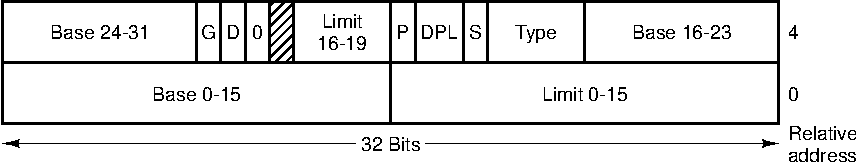
\includegraphics[width=.7\linewidth]{gdt}
  \caption{段描述符格式}
  \label{fig:gdt}
\end{figure}

图\ref{fig:gdt}所示为GDT的标准格式,GDT表就是根据该格式来进行配置
的。值得注意的是从\texttt{DESC\_DPL\_0}到\texttt{DESC\_DPL\_3}这四行代
码,它们代表的是保护模式特有的特权级概念。如图\ref{fig:tequan}所示,特
权级号越小权限越大,因此在进入保护模式后,操作系统的特权级应当是在0处,
而用户程序位于最低的特权级3处;若是实模式的话所有的一切都存在于同一个特
权级,这样实在是太危险了,所以这也是要费尽千辛万苦也要使操作系统进入保
护模式的原因之一。

\begin{figure}[H]
  \centering
  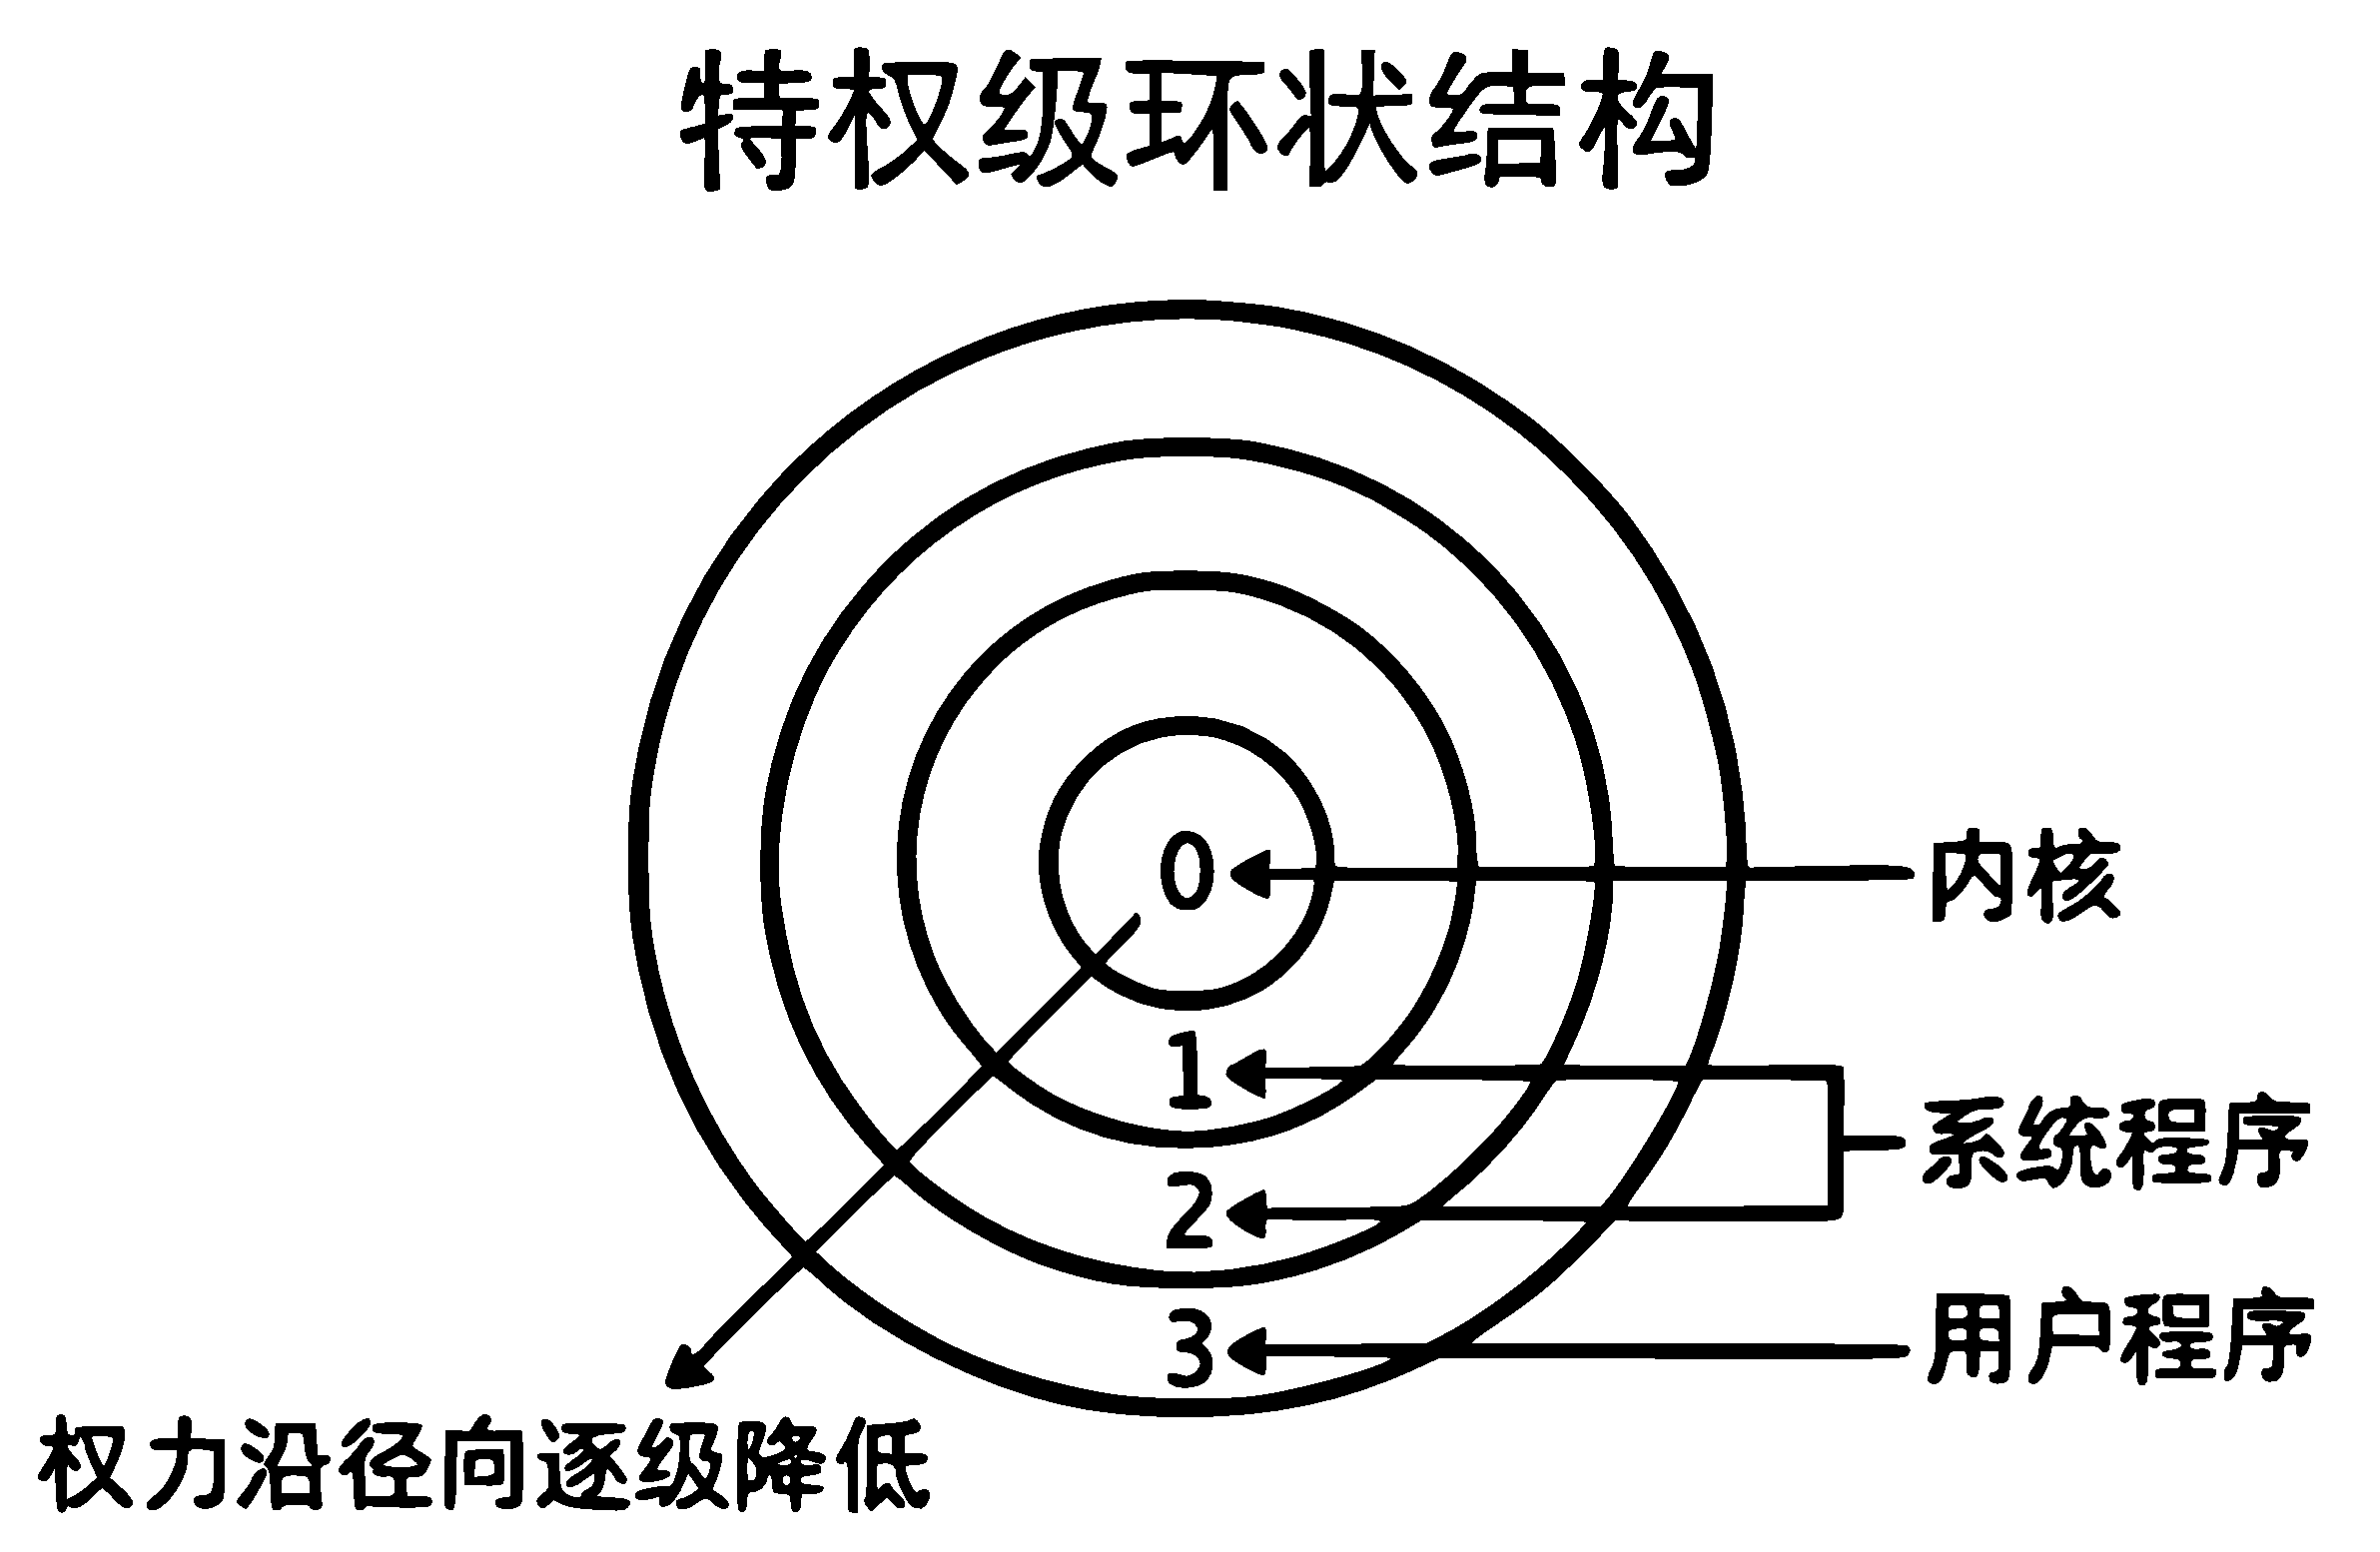
\includegraphics[width=.4\linewidth]{priv}
  \caption{特权级结构}
  \label{fig:tequan}
\end{figure}

关于A20地址线打开与否的区别:
\begin{itemize}
\item 如果A20地址线被打开,当访问到\texttt{0x100000~0x10FFEF}之间的地址时,CPU将真正访问到这块物理
  地址。
\item 如果A20地址线未被打开,当访问\texttt{0x100000~0x10FFEF}之间的地
  址时,CPU将采用8086/8088的地址回绕。实模式下的地址线是20位,最大寻址
  空间是1MB,即\texttt{0x00000~0xFFFFF}。超出1MB内存的部分在逻辑上虽然
  也是正常的,但物理内存中没有与之对应的部分,所以为了让“(段:偏移地
  址)”的策略可用,CPU会采取将超过1MB的部分自动绕回0地址的做法,继续
  从0地址开始映射,这就叫做地址回绕。如:\texttt{0x100000},由于没有第21位地址线,
  相当于丢掉了进位1,将会变成\texttt{0x00000}。
\end{itemize}

所以,在进入保护模式后就需要抛弃地址回绕这种做法,相应的也就需要超过20条地址去访问更大的空间,
而打开A20地址线就是以此为目的。最后,
\begin{codeblock}
  \begin{nasmcode}
    jmp dword SelectorCode32:0
  \end{nasmcode}
\end{codeblock}
将\texttt{CR0}寄存器的PE比特置1后,操作系统就成功的跳入了保护模式。

\subsection{加载内核}
\label{subsec:kernel}

在加载Kernel之前,得先获取物理内存容量,只有掌握了物理内存的大小,才能
更好地操作虚拟内存。在此,可以利用BIOS中断号\texttt{0x15}的子功能来获
取物理内存的大小。代码详见附录\ref{fsec:loader_15h}。其工作过程大致如下:
\begin{itemize}
\item 定义好调用之前输出的寄存器\texttt{ECX}和\texttt{EDX};
\item 调用int \texttt{0x15}号中断;
\item 在返回后输出的CF位为0时,寄存器\texttt{EAX}、\texttt{ES:DI}、\texttt{ECX}、
  \texttt{EBX}便会出现对应的结果。
\end{itemize}

如图\ref{fig:xp}所示,在执行\texttt{xp 0xB00}后,结果是\texttt{0x02000000},换算成十进制正好是32MB,故检测结果是正
确的。到这里SheepOS已经有了物理内存检测的功能,这下就能够对物理内存做到心中有数了。
虽然对物理内存的多少已经能够掌握了,但这些内存对于以后整个计算机而言还是太小了,在保护模式
中,地址空间达到了4GB,但目前是所有的进程包括操作系统共享这一个4GB,这样听起来就觉得
4GB其实也很小,所以还需要对内存进行分页。

\begin{figure}
  \centering
  \includegraphics[width=15cm]{图3-3}
  \caption{用xp命令查看物理内存}
  \label{fig:xp}
\end{figure}

图\ref{fig:fenye}所示是分页机制的工作原理,在打开分页机制后,原本的保护
模式的寻址方式又将改变,将从“(段选择子:段:偏移地址)”变成“(GDT:虚拟地址:页:物理地址)”
的寻址方式。因为有了分页机制后,就可以将线性地址转换成物理地址,且可以用
大小相等的页来代替大小不等的段,具体如图\ref{fig:fenyezy}所示。

\begin{figure}
  \centering
  \includegraphics[width=12cm]{图3-5}
  \caption{分页机制}
  \label{fig:fenye}
\end{figure}

\begin{figure}[H]
  \centering
  \includegraphics[width=12cm]{图3-4}
  \caption{分页机制的作用}
  \label{fig:fenyezy}
\end{figure}

虚拟地址与物理地址之间有一个映射关系,它们之间的转换是以页(4KB)为单位的。
一个页表有1024个页表项,一个页表项指向一个页的首地址,那4GB就需要1M个页,而一个页是
4KB,所以就需要1024个页表,也就是一个页表目录(二级页表)。而启用分页机制需要按顺序做3件事:
1)准备好页表目录和页表;2)将页表地址写入控制寄存器\texttt{CR3};3)寄存器CR0的PG比特置1。
页表目录和页表的创建过程大致如下:

\begin{itemize}
\item 需要先把页目录占用的空间逐字节清0;
\item 之后创建页目录项(PDE);
\item 再将页目录项0和0xc00都存为第一个页表的地址;
\item 创建页表项(PTE);
\item 创建内核其它页表的PDE;
\item 把页表地址写入CR3;
\item 将CR0的PG位置1;
\item 最后在开启分页后,用GDT新的地址重新加载;
\end{itemize}
代码详见附录\ref{fsec:loader_page}。

如图\ref{fig:infogdt},GDT的段基址已经变成了\texttt{0xc0000900},段描述符的段基址也变成\texttt{0xC00B8000},而
不是\texttt{0xB8000}了,说明SheepOS已经成功进入了分页机制的运行模式。
\begin{figure}[H]
  \centering
  \includegraphics[width=15cm]{图3-6}
  \caption{分页后GDT的变化}
  \label{fig:infogdt}
\end{figure}

接下来就该加载SheepOS的“心脏” --- 内核\cite{RL2011}了,加载内核到内存这一步跟MBR的工作基本
上都是同样的,首先第一步就是像把\texttt{Loader.bin}放到第4扇区那样把\texttt{Kernel.bin}放
到自己想放的位置上去,因为Loader在第4扇区上,第0扇区放的是MBR,最好给Loader多预留些位置,所
以在该操作系统中选择把\texttt{Kernel.bin}放到第7扇区,确定好要放的扇区的位置后,可以直接用dd命令往磁盘上写:

\begin{shellcode}
dd if=kernel.bin of=/SheepOS/hd60M.img bs=512 count=200 seek=7 conv=notrunc  
\end{shellcode}

\begin{itemize}
\item \texttt{seek}为7,目的是越过前7个扇区(第0 \char`~{} 6个扇区),
  在第7个扇区写入内核。
\item \texttt{count}为200,目的是一次往参数\texttt{of}指定的文件中写
  入200个扇区。
\end{itemize}

这样,\texttt{Kernel.bin}就被成功的写入磁盘了,接下来就该让Loader去找
到Kernel然后把它从硬盘上搬运到内存中去,跟之前MBR搬运Loader一样,还需要
一个缓冲区,如图\ref{fig:hc}所示,跟之前Loader一样,有两个可用区域,
准确的说是三个,因为现在MBR也结束任务了,所以之前MBR所占用的区域现
在也可以使用。

\begin{figure}[H]
  \centering
  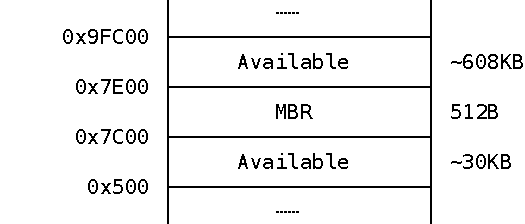
\includegraphics[width=.4\linewidth]{boot-mem2}
  \caption{可用缓冲区}
  \label{fig:hc}
\end{figure}

之后内核文件会越来越大,所以,为了能够预留出足够的空间,需要将\texttt{Kernel.bin}
加载到地址较高的空间,但内核映像要放置在较低的地址中,因为\texttt{Kernel.bin}在被
Loader加载之后就没用了,之后,内核映像在向高地址处扩展的时候也可以覆盖之前加载到高地址的
\texttt{Kernel.bin}所占用的空间。所以该操作系统中把Kernel加载到了\texttt{0x70000}这个地址\cite{DM2006}
。Loader加载Kernel到内存的
代码如下:

\begin{nasmcode}
   KERNEL_START_SECTOR equ 0x200
   KERNEL_BIN_BASE_ADDR equ 0x70000
   mov eax, KERNEL_START_SECTOR        ; kernel.bin所在的扇区号
   mov ebx, KERNEL_BIN_BASE_ADDR       ; 从磁盘读出后,写入到ebx指定的地址
   mov ecx, 200                ; 读入的扇区数

   call rd_disk_32
\end{nasmcode}

其中,\texttt{0x200}就是为\texttt{Kernel.bin}设置的地址,\texttt{0x70000}是Loader在\texttt{0x200}找到\texttt{Kernel.bin}后加载到的地址。
在Loader把Kernel加载到\texttt{0x70000}之后,还需要对内核进行一下初始化
(程序代码参见附录\ref{fsec:kernel_init}),其过程大致如下:
\begin{itemize}
\item 将\texttt{kernel.bin}中的段拷贝到各个段自己被编译的虚拟地址处;
\item 把这些段单独提取到内存中;
\item 判断段类型,如果不是\texttt{PT\_NULL},就把这些段拷贝到编译的地址中。
\end{itemize}

至此,SheepOS已经成功拥有内核了,且之后CPU的控制权也将交给内核。


%%% Local Variables:
%%% mode: latex
%%% TeX-master: "../thesis"
%%% End:
